  %**************************************************************
% Telemanom
%**************************************************************

\subsection{Telemanom} \label{sez-telemanom}
    Telemanom\cite{telemanom} è una tecnica di rilevazione di anomalie sviluppata dai ricercatori della Nasa nel 2018 
    ai fini dell'anomaly detection su stazioni e veicoli spaziali. Il modello è stato applicato dai ricercatori sui 
    dati telemetrici dei satelliti e del rover Curiosity e, come MSCRED\cite{mscred}, utilizza reti neurali 
    Long-Short Term Memory (LSTM\cite{convlstm}).

    La scelta di utilizzare Telemanom in questa ricerca si è basata sulla necessità di confrontare MSCRED con un modello 
    più recente che sfrutta tecniche avanzate focalizzate sull'apprendimento profondo, concentrandosi esclusivamente 
    sulla rilevazione delle anomalie.

    Il modello nasce come miglioramento ai vecchi sistemi di anomaly detection per l'attrezzatura spaziale 
    che, in generale, erano semplicemente basati su valori precisi e predeterminati che, una volta superati, facevano sì che venissero
    attivate le misure di sicurezza opportune. Telemanom è stato progettato tenendo presente che i dati vivono in un 
    contesto non supervisionato ed è in grado di osservare segnali multipli e analizzare se un certo canale (segnale)
    si trova in uno stato anomalo o meno individualmente dagli altri segnali. Questo permette di tracciare più facilmente 
    le cause dell'anomalia. Per cui Telemanom tratta un contesto ancora più complesso rispetto a quello in cui vive InfoSapienza, 
    dove le anomalie sono globali per tutti i segnali.

    \paragraph{Intuizione} Telemanom effettua previsioni creando un modello distinto per ciascun canale di telemetria,
    questo significa che ogni canale viene trattato in modo indipendente per la previsione. Il modello
    viene addestrato per predire un certo numero di valori futuri per ciascun canale di telemetria. Durante il 
    processo di previsione, l'errore attuale di previsione $e(t) = y(t) - \hat{y}(t)$, in cui $y(t)$ è il valore 
    ground-truth mentre $\hat{y}(t)$ è il valore previsto dal modello, viene smussato attraverso una media 
    ponderata esponenziale. L'insieme degli errori smussati forma un vettore $\mathbf{e}_s$. 
    
    Dato il vettore $\mathbf{e}_s$, la soglia di anomalia è calcolata attraverso un approccio che identifica i valori estremi 
    senza supposizioni sulla distribuzione degli errori. 
    Il threshold $\epsilon$ è calcolato come segue: 
    $\epsilon = \mu(\mathbf{e}_s) + \mathbf{z}\sigma(\mathbf{e}_s)$ in cui $\mathbf{z}$ è una lista ordinata di valori 
    positivi che rappresentano il numero di deviazioni standard sopra la media $\mu(\mathbf{e}_s)$. 

    Sia il vettore $\mathbf{e}_{seq}$ che rappresenta gli errori smussati i cui valori $e^{(i)} \geq \epsilon$, 
    ovvero è un vettore che contiene tutti gli errori smussati che hanno il proprio valore maggiore al valore di threshold, la severità 
    dell'anomalia $s^{(i)}$ per ogni punto è calcolata come segue:

    \[s^{(i)} = \frac{\max(\mathbf{e}_{seq}^{(i)}) - \arg \max(\epsilon)}{\mu(\mathbf{e}_s) + \sigma(\mathbf{e}_s)}\]

    Il rilevamento di anomalie basato sulla previsione dipende in modo significativo dai dati storici utilizzati
    per calcolare la soglia dinamicamente e valutare gli errori di previsione correnti. Da ciò deduciamo che la 
    mancanza di dati storici può portare a falsi positivi che sono calcolati anomali solo a causa del contesto ristretto 
    in cui essi vengono valutati. Telemanom risolve questo problema applicando una procedura di pruning atta a mitigare 
    i falsi positivi e assume che le anomalie di dimensione simile di solito non si verificano frequentemente 
    nello stesso canale. Queste accortezze aiutano a migliorare la precisione del modello, contribuendo a considerare
    i comportamenti normali ma rari delle attrezzature spaziali che si verificano a intervalli regolari.

    \paragraph{Dataset} Telemanom, come già enunciato, prende in considerazione un unico canale alla volta. È 
    quindi necessario suddividere il dataset di Infostud in più parti, una per ogni segnale, per far sì che il modello 
    venga addestrato ed effettui previsioni su tutto il dataset. Gli intervalli anomali associati a ogni canale sono gli 
    stessi, poiché nel caso di InfoSapienza quando avviene un'anomalia, essa è globale per tutti i servizi, quindi 
    per tutti i segnali.

    Per l'esperimento è stato utilizzato lo stesso dataset applicato ai modelli precedenti e discusso nel 
    \hyperref[cap2]{Capitolo 2}, ma il cui indice di split è diverso rispetto ai modelli 
    precedentemente analizzati. Questo perché Telemanom, in generale, prevede un'anomalia se il modello osserva come anomalo 
    l'intervallo in cui l'anomalia si verifica. Le varie metriche, nell'implementazione originale che è stata 
    utilizzata per gli esperimenti, vengono quindi basate solo sugli intervalli considerati anomali, non sul numero 
    di punti previsti come anomali come nelle altre applicazioni analizzate. Il dataset di Infostud preso in 
    analisi ha complessivamente cinque intervalli di anomalie distinte e, se prendessimo 
    in considerazione lo split analizzato precedentemente, solo uno sarebbe nell'insieme di test. Per far sì che il modello 
    sia addestrato e testato in maniera più egregia, è stato scelto lo split osservabile nella 
    \hyperref[tab:dataset-telemanom]{Tabella 3.4.} Il dataset suddiviso è illustrato nella \hyperref[fig:telemanom-data]{Figura 3.6.}, 
    mentre la \hyperref[fig:telemanom-train]{Figura 3.7.} mostra il dataset di addestramento della metrica che 
    rappresenta la latenza media delle richieste di login a InfoSapienza.

    \begin{table}[H]
        \centering
        \caption{Statistiche dataset Telemanom.}
        \begin{tabular}{lccc}
            \toprule
            \textbf{Dataset} & \textbf{Indice di split} & \textbf{\# punti} & \textbf{\# Intervalli anomali} \\
            \midrule
            \textbf{Training} & 0.43 & 20784  & $3$ \\
            \textbf{Testing} & 0.67 & 27553 & $2$ \\
            \bottomrule
        \end{tabular}
        \label{tab:dataset-telemanom}
    \end{table}

    \begin{figure}[H]
        \centering
        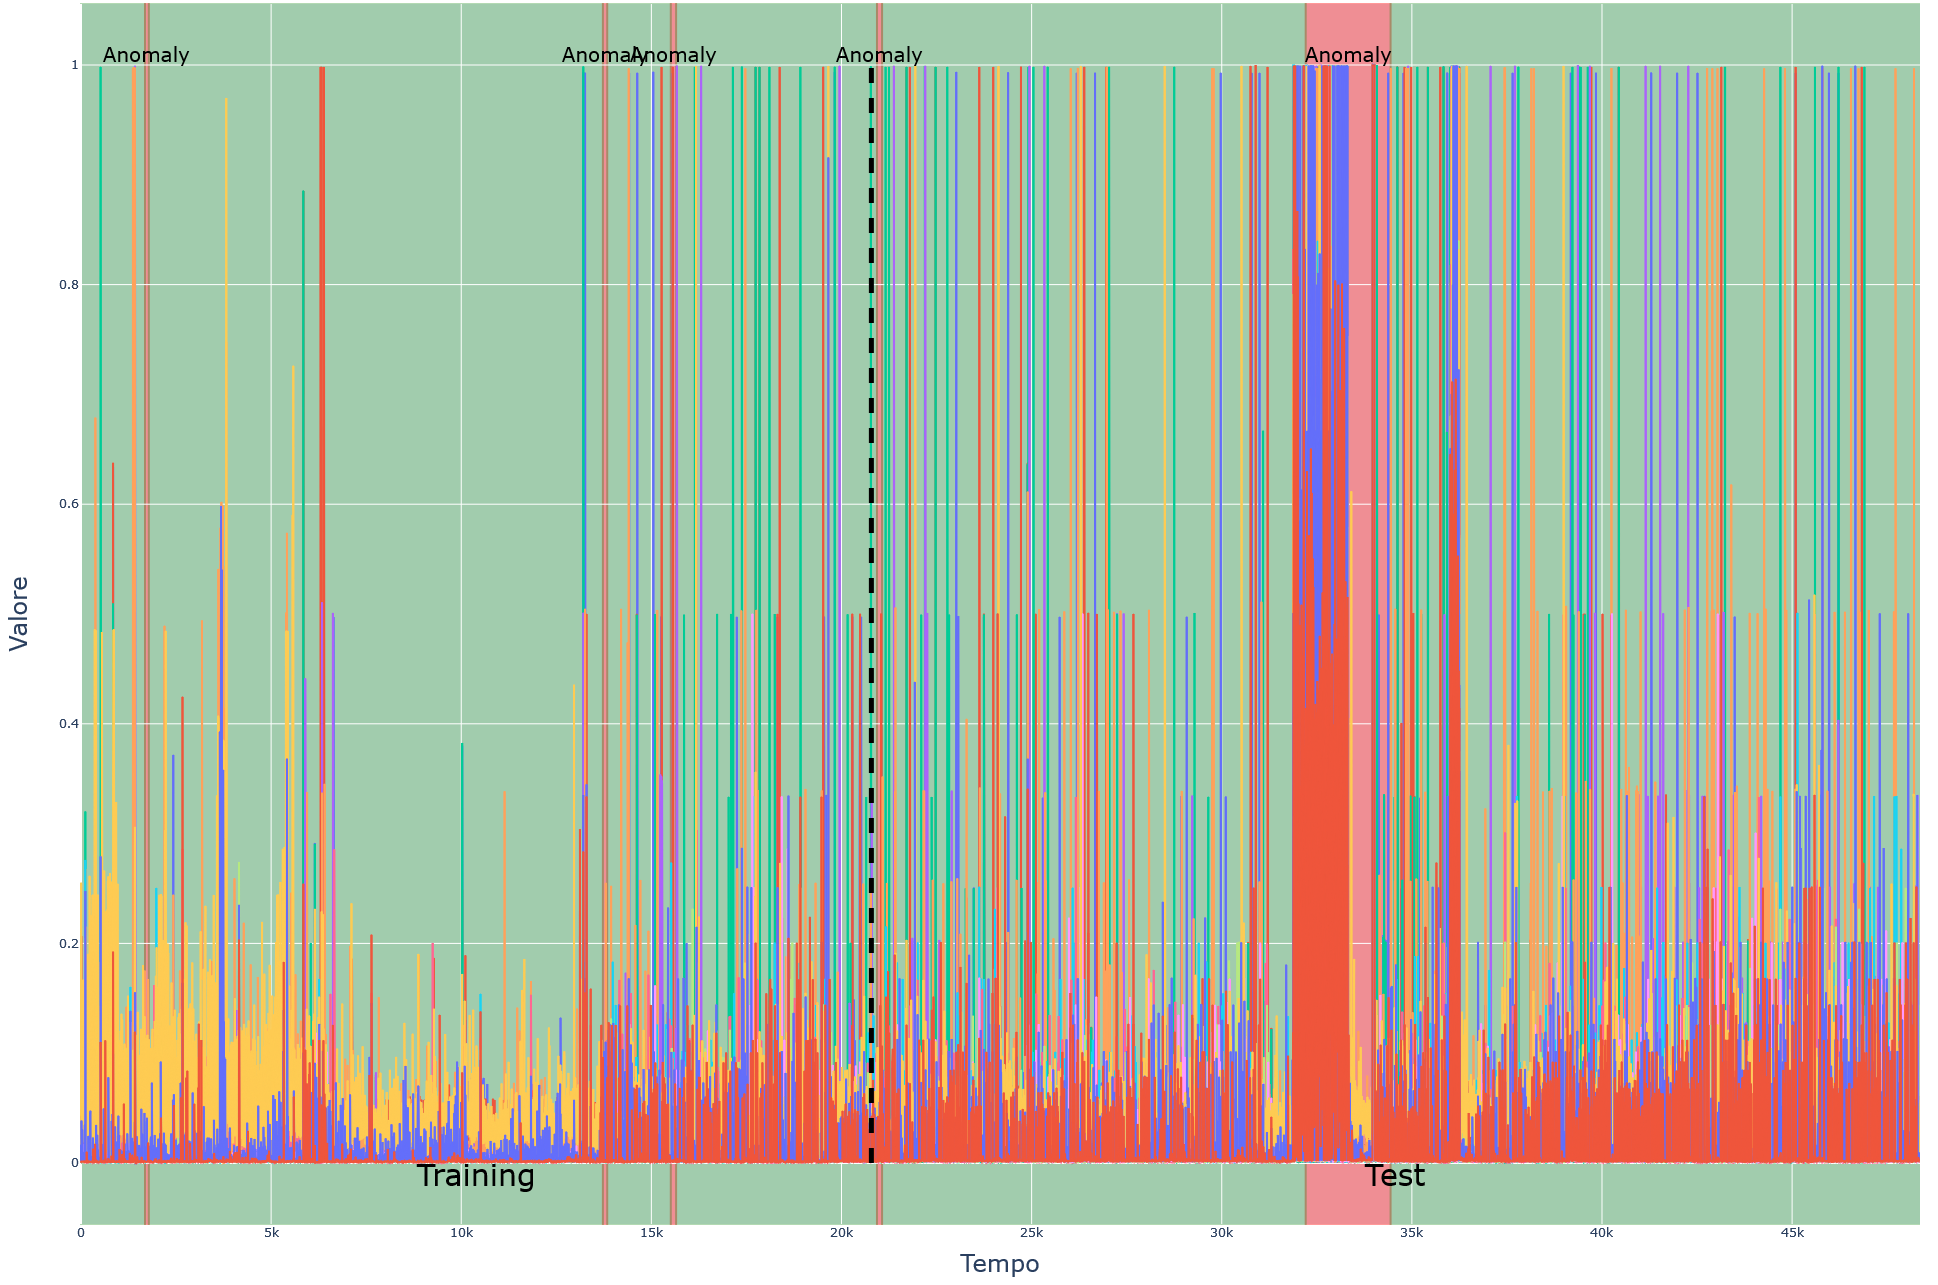
\includegraphics[width=0.6\textwidth]{./input/chapters/models/figs/telemanom-data.png}
        \caption{Suddivisione dataset negli insiemi di training e test. La linea tratteggiata delimita il dataset 
        di training da quello dedicato al test.}
        \label{fig:telemanom-data}
    \end{figure}

    \begin{figure}[H]
        \centering
        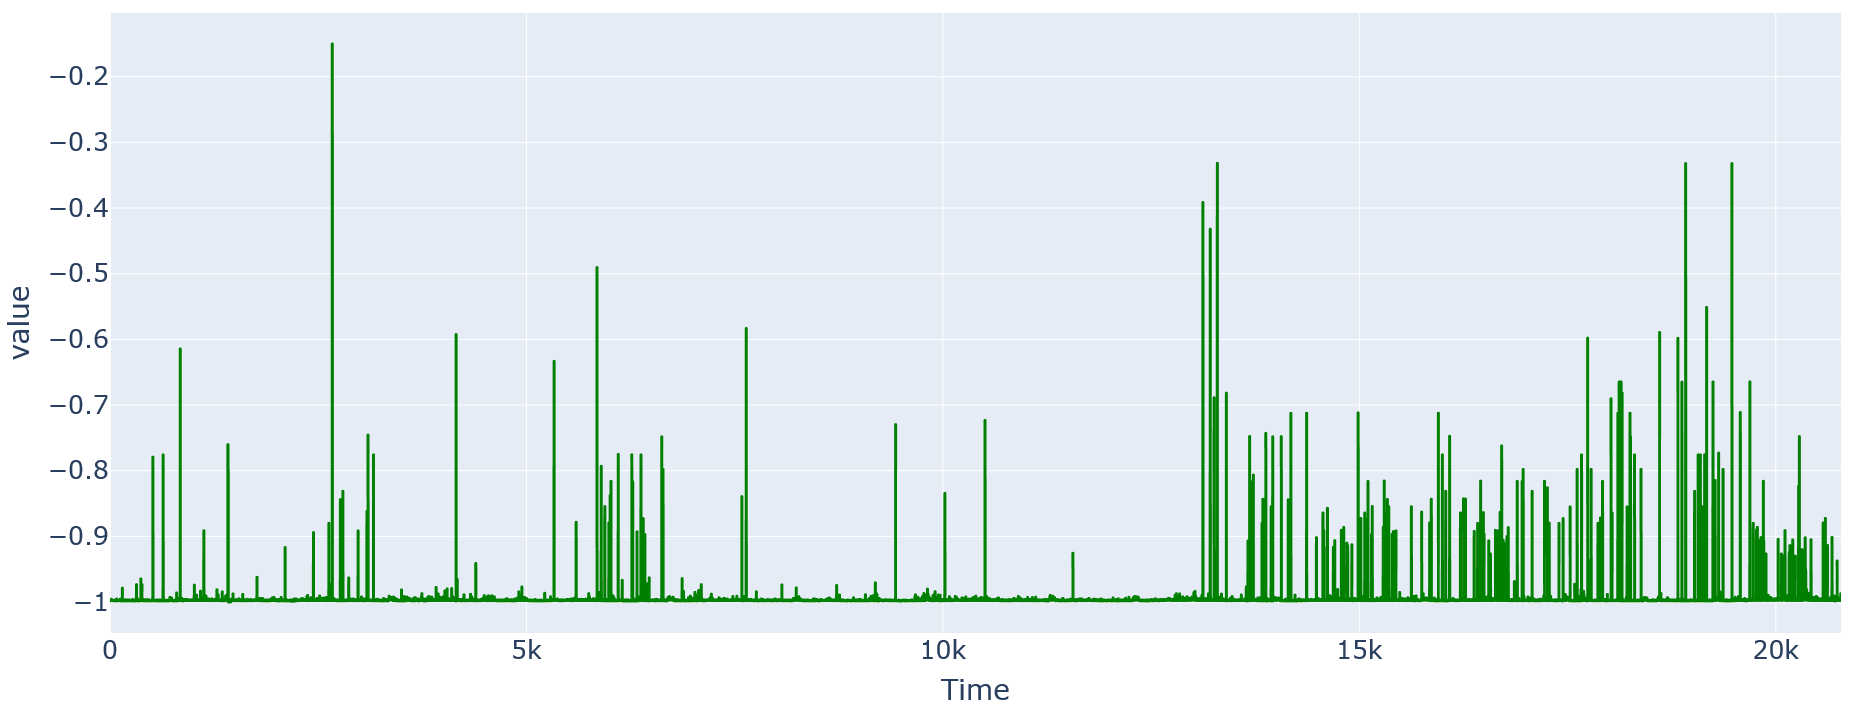
\includegraphics[width=0.7\textwidth]{./input/chapters/models/figs/telemanom-train-data.png}
        \caption{Insieme di training di Telemanom.}
        \label{fig:telemanom-train}
    \end{figure}

    Non è stato necessario assicurare una parte di dati al validation set perché Telemanom, nella sua 
    implementazione, gestisce da sé la validazione per l'addestramento della sua rete neurale.

    \paragraph{Iperparametri} Telemanom presenta numerosi iperparametri, tra i quali i più significativi sono riportati nella
    \hyperref[tab:telemanom-hyperparams]{Tabella 3.5.}, insieme ai valori empiricamente scelti per questo esperimento.
        
    \begin{table}[H]
        \centering
        \caption{Descrizione e valori degli iperparametri Telemanom.}
        \begin{tabular}{p{0.25\linewidth}p{0.55\linewidth}p{0.10\linewidth}}
            \toprule
            \textbf{Iperparametro} & \textbf{Informazioni} & \textbf{Valore}\\
            \toprule
            $batch\_size$ & Indica il numero di valori da considerare in ogni batch durante l'addestramento. & $100$\\
            \midrule
            $window\_size$ & Specifica il numero di batch precedenti da utilizzare nel calcolo dell'errore smussato.  & $110$\\
            \midrule
            $smoothing\_perch$ & Determina l'indice di smussamento nel calcolo degli errori. & $0.1$ \\
            \midrule
            $layers$ & Vettore bidimensionale che rappresenta il numero di neuroni negli strati nascosti della rete neurale. & $[100,100]$\\
            \midrule
            $l_s$ & Numero di passi temporali precedenti a quello attuale su cui verrà basata la previsione futura. & $7$ \\
            \midrule
            $n\_predictions$ & Indica il numero di valori futuri da prevedere. & $35$ \\
            \midrule
            $validation\_split$ & Specifica la percentuale del dataset di training che verrà usato come validazione per l'addestramento 
                della rete neurale. & $0.2$\\
            \bottomrule
        \end{tabular}
        \label{tab:telemanom-hyperparams}
    \end{table}

